\documentclass[12pt,a4paper]{article}
\usepackage{tabularx}
\usepackage{booktabs}
\usepackage{longtable}
\usepackage{ltxtable}
\usepackage[latin1]{inputenc}
\usepackage{amssymb}
\usepackage[]{graphicx,rotating}
\usepackage[T1]{fontenc}
\usepackage{parskip}
\usepackage{listings}
\usepackage{natbib}
\usepackage[official]{eurosym}
\usepackage{mathrsfs}
\usepackage{amsmath}
\usepackage{verbatim}
\usepackage[usenames,dvipsnames]{color}     %for R colors and formatting

\usepackage[left=3cm, right=2.5cm, top=2.5cm]{geometry}

\pagestyle{empty}
\parindent 0cm
\renewcommand{\baselinestretch}{1}
\newcommand{\bs}{\boldsymbol}
\renewcommand{\familydefault}{cmr}
\pdfminorversion=7
\bibliographystyle{agsm}

\lstset{ %for R colors and formatting
  language=R,                     % the language of the code
  basicstyle=\scriptsize\ttfamily, % the size of the fonts that are used for the code
  numbers=left,                   % where to put the line-numbers
  numberstyle=\scriptsize\color{Blue},  % the style that is used for the line-numbers
  stepnumber=1,                   % the step between two line-numbers. If it is 1, each line
                                  % will be numbered
  numbersep=5pt,                  % how far the line-numbers are from the code
  backgroundcolor=\color{white},  % choose the background color. You must add \usepackage{color}
  showspaces=false,               % show spaces adding particular underscores
  showstringspaces=false,         % underline spaces within strings
  showtabs=false,                 % show tabs within strings adding particular underscores
  frame=single,                   % adds a frame around the code
  rulecolor=\color{black},        % if not set, the frame-color may be changed on line-breaks within not-black text (e.g. commens (green here))
  tabsize=2,                      % sets default tabsize to 2 spaces
  captionpos=b,                   % sets the caption-position to bottom
  breaklines=true,                % sets automatic line breaking
  breakatwhitespace=false,        % sets if automatic breaks should only happen at whitespace
  keywordstyle=\color{RoyalBlue},      % keyword style
  commentstyle=\color{YellowGreen},   % comment style
  stringstyle=\color{ForestGreen}      % string literal style
} 

\begin{document}

\begin{center}
% \vspace*{1cm}
 
\includegraphics[width=0.35\textwidth]{GU-Logo-blau-CMYK.eps} \vspace{2cm}
  
  {\Large{\bf Estimating Profit-optimal Nash Equilibrium Market Shares and Prices for the Beer Market}} \medskip

  {\Large{Hierarchical Bayesian MNL Models in a Dynamic Market Environment}} \vspace{0.5cm}

  Term Paper \\\vspace{2cm}
  submitted to \\\vspace{0.5cm}
  \textbf{Prof. Dr. Thomas Otter} \\\vspace{0.5cm}
  Goethe University Frankfurt am Main \\
  School of Business and Economics \\
  Chair of Services Marketing \vspace{2cm}
  
  by \\\vspace{0.5cm}
  \textbf{Lukas J\"urgensmeier} \\
  (Mat.-Nr.: 6904281) \\
  
  \bigskip

  in partial fulfillment of the requirements of the lecture \medskip

 {\bf Customer Satisfaction and Consumer Choice} \\
  Summer Semester 2019\\
  \medskip

  July 23, 2019
  
\end{center}


\pagebreak
\pagestyle{plain}
\pagenumbering{Roman}
\tableofcontents
\pagebreak
\listoffigures
\pagebreak
\listoftables
\newpage
\setcounter{page}{2}
\pagenumbering{arabic}
\setlength{\baselineskip}{1.5\baselineskip}
\pagestyle{plain}


\section{Contextual Introduction to the Beer Market}
\begin{itemize}
\item Beer market description: Find market study that describes competitive situation
\item Prices, Competition, Profits, Marginal Costs
\item Recent developments in the beer market (market power of few breweries)
\item Is it the Spanish beer market?
\end{itemize}

\section{Motivation of the Analytical Model}
Historically, marketing research has heavily relied on Conjoint Analysis.
It is a tool to measure consumers' preferences in a more realistic way by asking them to choose between different products that imply trade-offs.
This is a method to derive consumers' preferences in a more credible way than to ask them which brand or feature they prefer,
since this often yields trivial results\footnote{i.e. preferring the cheap vs. the expensive good or valuing the better quality good more than the low quality product.}.
Choice-based Conjoint data enables researchers to calculate counterfactual scenarios, such as what happens to a company's market share if a competitor changes its price.
To analyze choice-based Conjoint data, market research has focused on the Multinomial Logit (MNL) Model.
Unfortunately, the MNL model is based on two strong assumptions.
First, choices should be independent of irrelevant alternatives (IIA).
This means that consumers' choices are not influenced by the presence or absence of another, supposedly irrelevant other choice option.
However, numerous examples have been constructed to easily show that this assumption is often violated, most famously the blue and red bus example by \cite{mcfaddenConditionalLogitAnalysis1973}.
Especially for substitute products, this assumtion therefore does not hold. 
Modeling very similar choices with a traditional MNL model is hence not desirable.
The second strong assumption that is required for MNL estimation is homogeneity in preferences across consumers.
This implies that consumers' preferences---expressed by the beta estimates---are identical, which does not hold in reality. 

Literature has acknowledged those violations and proposed the heterogeneous MNL, a more flexible model that relaxes the IIA assumption \citep{steckelHeterogeneousConditionalLogit1988}.
As a remedy to the second critical assumption's violation, hierarchical MNL models allow for differences in consumer preferences.

When taking those beta coefficients to simulate individual choices as well as aggregate market outcomes and equilibrium prices,
standard approach was to assume that all prices in the choice set were within the consumer's unobserved budget.
\cite{pachaliPerilsIgnoringBudget2017} argue that this simplification leads to a serious over-estimation of equilibrium prices.
They claim that it still holds if priors such as sign constraints are included and reasonably specified in the estimation such as in \cite{sonnierHeterogeneityDistributionsWillingnesstopay2007} and \cite{allenbyEconomicValuationProduct2014}.
Instead of "cleaning" the data until derived estimates mirror the desired price ranges, this paper follows \cite{pachaliPerilsIgnoringBudget2017}
and applies a hierarchical Bayes model which is capable of inferring previously unobserved budgets, additionally to sign constraints for $\beta_{price}$.
This study applies the indirect utility model by \cite{berryAutomobilePricesMarket1995}.
It is superior to the price screening model proposed by \cite{gilbrideChoiceModelConjunctive2004},
since its models a continuous choice probability dependent on price.
Logit choice probabilities need to be continuous at every draw in order to derive a pure-strategy Nash equilibrium \citep{morrowFixedPointApproachesComputing2011, pachaliPerilsIgnoringBudget2017}.

Concluding this section, the analytical model implemented in this study addresses three serious shortcomings of most common methods to conduct a market simulation and derive profit-maximizing prices.
It relaxes the IIA assumption, allows for heterogeneous individual-level consumer preferences, and infers previously unobserved budgets.
Those three model specifications are believed to yield more realistic and less biased estimates \citep{chandukalaChoiceModelsMarketing2008, pachaliPerilsIgnoringBudget2017}.


\section{Exogenous Variables and Expected Relationships}

While the previous section motivated the analytical model and introduced model extensions to relax unrealistic assumptions,
this part introduces the empirical application of those tools.
This paper analyzes a Choice-based Conjoint data set for choices among different beer brands obtained by the market research institute Kantar TNS.
The data set recorded preferences for canned beer.
 $N=407$ respondents participated in the study and choose among $p=10$ alternatives per choice task (nine beer brands and one outside option).
Every participant performed $t=15$ choice tasks. In total, 15 distinct beer brands and one outside alternative were included in the study,
while the subjects were only presented with a subset of $p$ alternatives, always including the outside choice.
The data set consists multiple brands of the same brewery---four Amstel beers and two Estrella and Mahou beers each.
The remaining seven beer brands based on their brand names are assumed to belong to different companies.
Additionally to the beers' brand names, the price was displayed to the subjects, which ranged from 0.22 to 0.74\euro.

Consistent with economic theory, there should be a negative relationship between price and demand.
This is empirically analyzed in section \ref{sec_marketsim} and visually displayed in figure \ref{fig_scatter_brand_comp}.


\section{Model Description and Results}
Model
\begin{itemize}
\item $N=407$ respondents
\item $p=10$ choice tasks per respondent
\item Constraints: Only positive beta coefficient for price and budget. If we had negative price coefficients, there would be a negative reward in the BLP formula for saving portions of the budget
\item Budget constraints are inferred by consumer choices and max/min price chosen
\end{itemize}

Results
\begin{itemize}
\item present histograms of beta coefficients
\item discuss the means of beta coefficients: The higher it is, the more preferably the brand is, on average.
\item Look at standard deviations: Get an idea about how heterogeneous/homogeneous the preferences are
\item Get an insight about price sensitivity: Higher beta coefficient means less price sensitivity (stemming from preferences, not price coefficient)
\end{itemize}

\begin{figure}[ht]
	\centering
  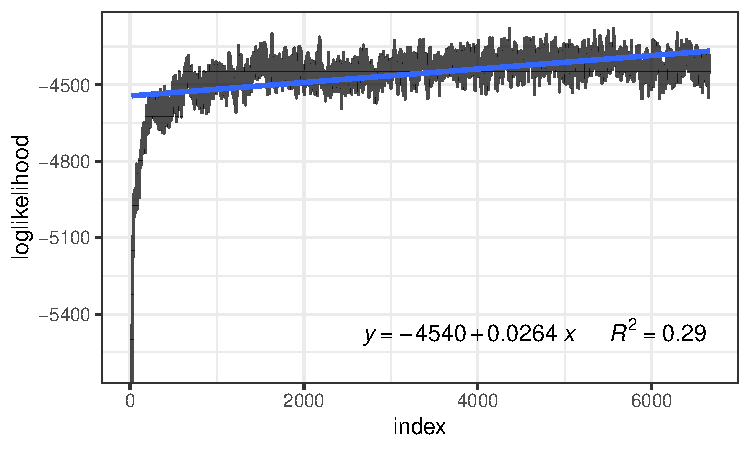
\includegraphics[]{figures/mcmc_before_burnin_fitted.pdf}
	\caption{Loglikelihood values of the MCMC routine with 100,000 iterations, keeping every 15\textsuperscript{th} value}
	\label{fig_mcmc}
\end{figure}

\begin{figure}[ht]
	\centering
  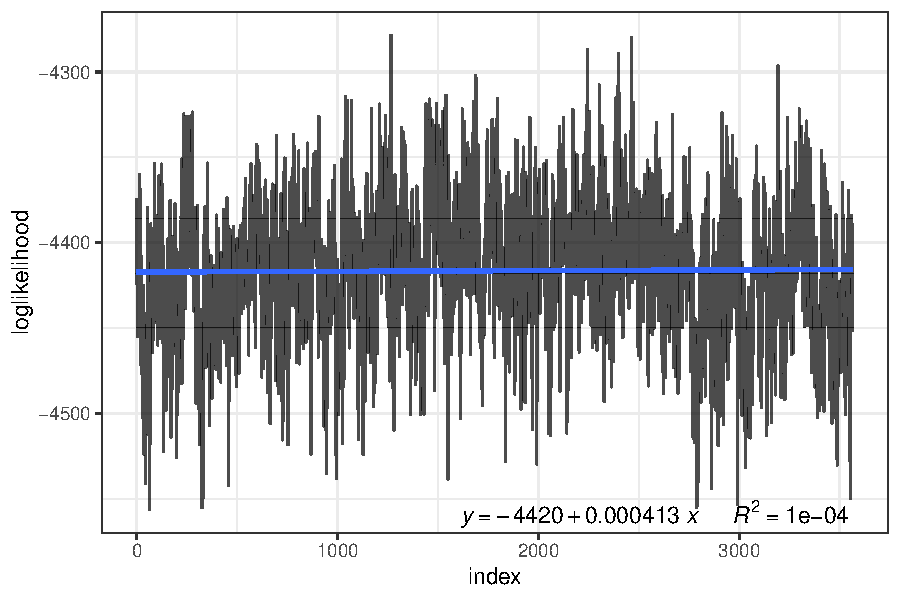
\includegraphics[scale = 0.8]{figures/mcmc_after_burnin_fitted.pdf}
	\caption{Loglikelihood values of the MCMC routine, after removing the first 3,100 observations}
	\label{fig_mcmc_burnin}
\end{figure}

\begin{figure}[ht]
	\centering
  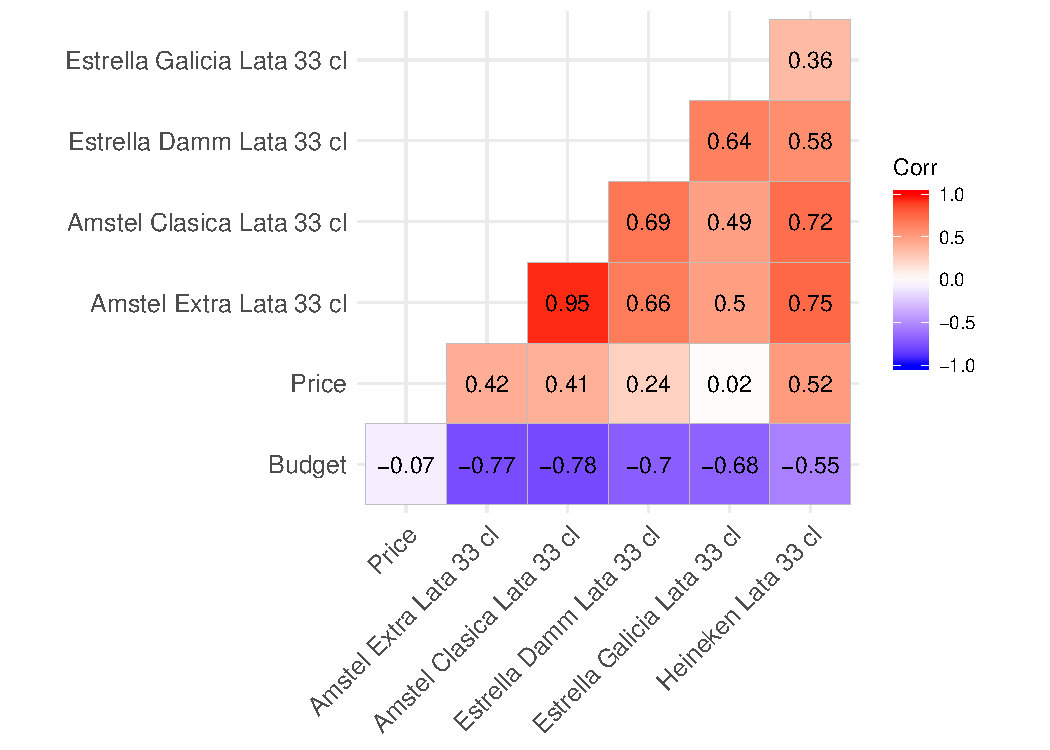
\includegraphics[scale = 0.7]{figures/corrplot_betas_five.pdf}
	\caption{Correlation of betas for price, budget and five brands}
	\label{fig_corr_five}
\end{figure}

\begin{figure}[ht]
	\centering
  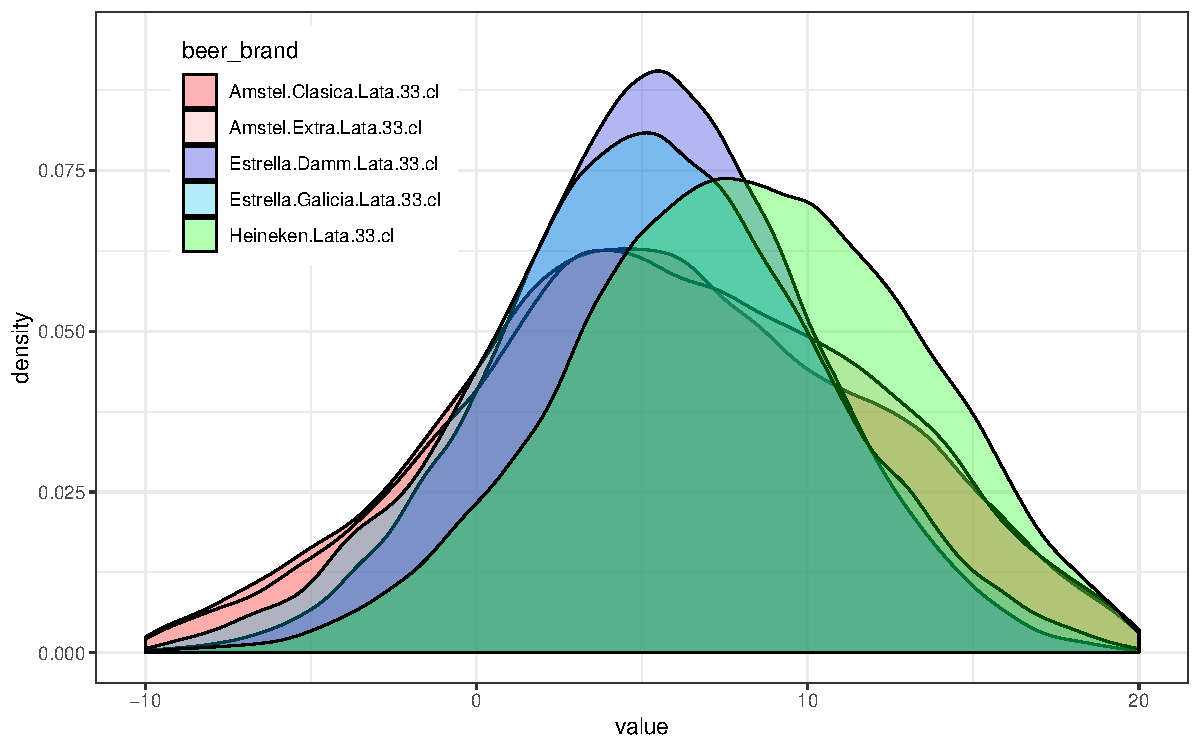
\includegraphics[scale = 0.6]{figures/dens_betas_five_in_one.pdf}
	\caption{Density plot for betas of five distinct brands}
	\label{fig_dens_five}
\end{figure}

\section{Market Simulation} \label{sec_marketsim}
\begin{itemize}
\item Assumptions about absolute marginal costs (e.g. 0.2 \euro). We assume it's not proportional to price and constant for all different brands.
\item Start with small set of brands (e.g. 3 Amstel beers + 1 outside)
\item Same ownership, which means monopoly
\item In a second step, we model a duopoly with same brands as before and one additional competitor (e.g. two Estrella brands)
\item If computationally feasible, we model all 15 beer brands in the same model (full competition, complete market)
\item Compute profit for each scenario by\\
 $Profit = (Equilibrium\ Price - MC)* Market\ Share$
\item Think about mergers: Vary ownership structure, e.g. we're Amstel and we buy Heineken. What does that do to Amstel's profits and market share?
\end{itemize}

\begin{figure}[ht]
	\centering
  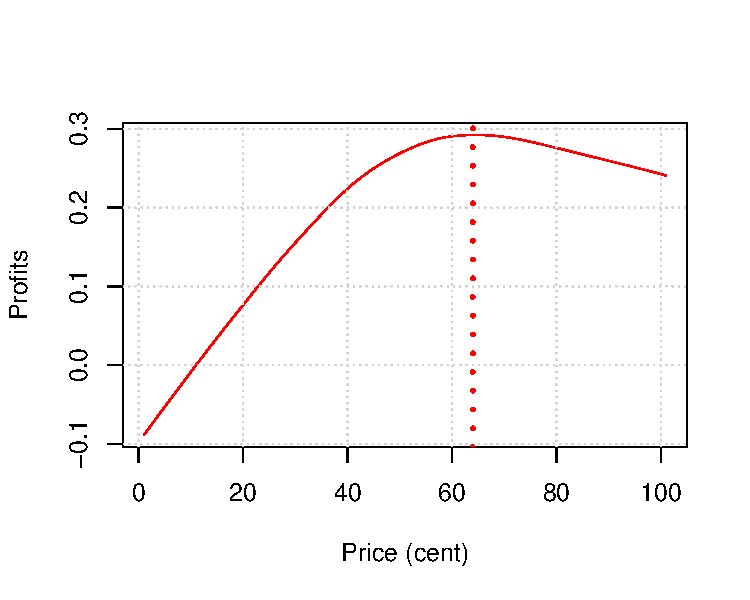
\includegraphics[scale = 0.7]{figures/opt_price_one_brand_static_monopoly.pdf}
	\caption{Price--profit curve in a static, one-brand monopoly market and profit-maximizing price (dashed vertical line)}
	\label{fig_opt_monopoly}
\end{figure}

\begin{figure}[ht]
	\centering
  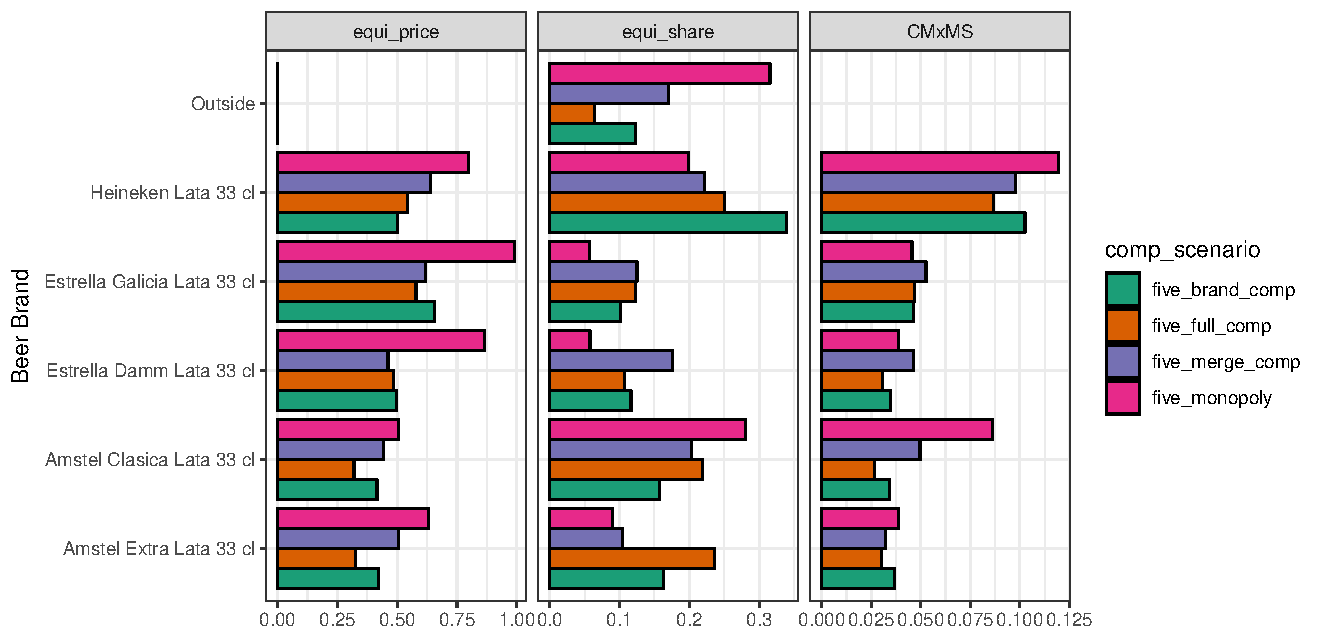
\includegraphics[scale = 0.7]{figures/bar_price_share_brand_merge_5.pdf}
	\caption{Prices and market shares in a profit-maximizing Nash equilibrium for five brands and outside option in a brand competition vs. merge setting}
	\label{fig_bar_five}
\end{figure}

\begin{figure}[ht]
	\centering
  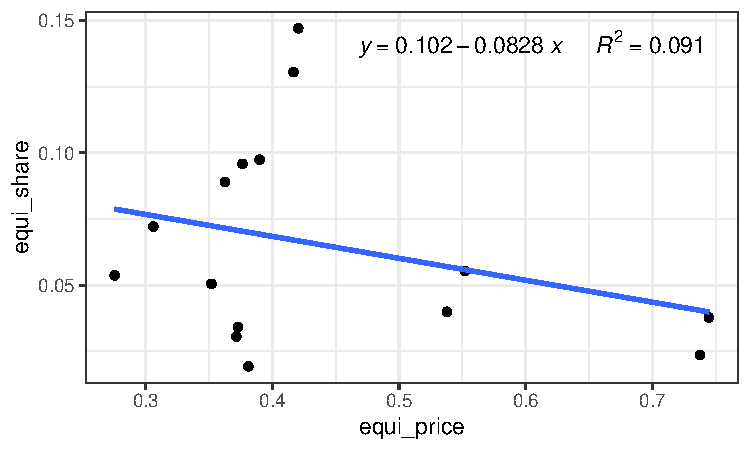
\includegraphics[scale = 0.7]{figures/scatter_price_share_brand_comp_fitted.pdf}
	\caption{Price--Market Share scatter plot with linear regression model fit}
	\label{fig_scatter_brand_comp}
\end{figure}

\section{Managerial and Research Implications}
\begin{itemize}
\item Take results from market simulation and derive managerial implications
\item E.g. take out product with the lowest market share and check if market share and profits of remaining products from our brand increases
\item Tool to determine if a merger would be beneficial
\end{itemize}

\clearpage
\appendix
\section{Figures}
\begin{figure}[ht]
	\centering
  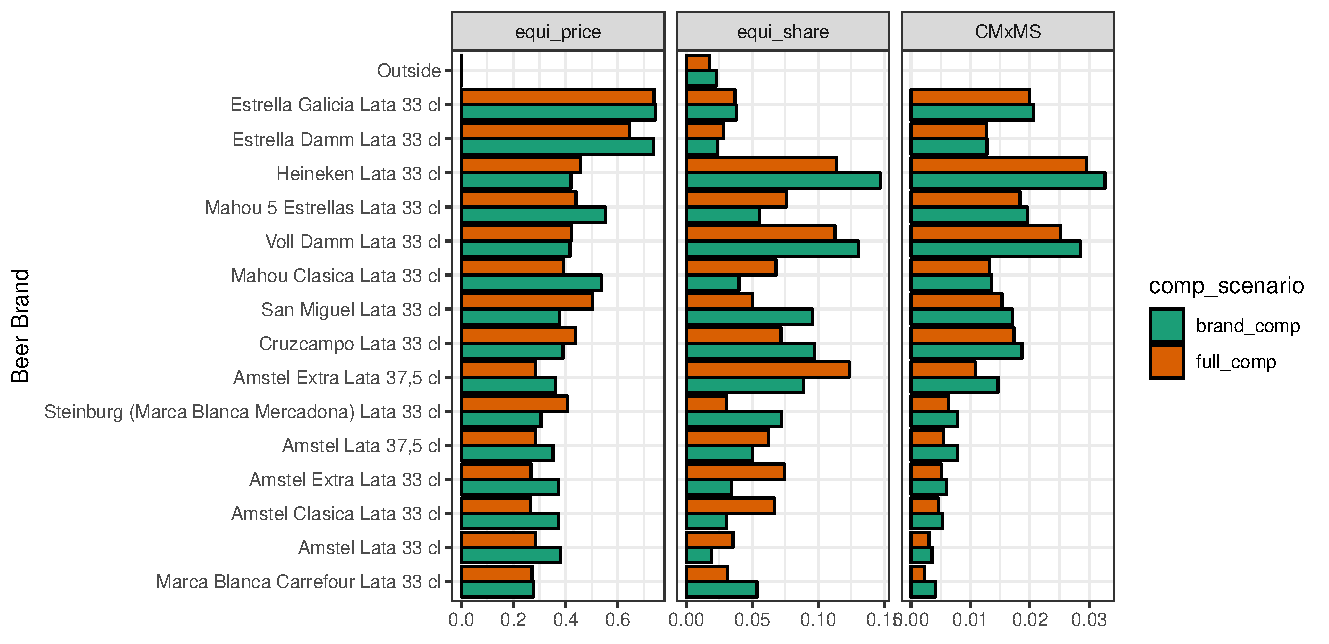
\includegraphics[scale = 0.7]{figures/bar_price_share_full_brand_15.pdf}
	\caption{Prices and market shares in a profit-maximizing Nash equilibrium for all 15 brands and outside option in a full vs. brand competition setting}
	\label{fig_bar_fifteen}
\end{figure}

\section{R Code}

\begin{lstlisting}[language=R,caption={Estimation Code}, label=lst:estim]


\end{lstlisting}


\clearpage
\bibliography{library}

\newpage
\thispagestyle{empty}
\section*{Statutory Declaration}

I herewith declare that I have completed the present term paper independently, without making use of
other than the specified literature and aids. Sentences or parts of sentences quoted literally are
marked as quotations; identification of other references with regard to the statement and scope of
the work is quoted. The thesis in this form or in any other form has not been submitted to an examination body and has not been published.
This thesis has not been used, either in whole or part, for another examination achievement.

\vspace{1cm}

Frankfurt am Main, July 23, 2019
\vspace{2cm}

. . . . . . . . . . . . . . . . . . . . . . . . . . . . . . .
\vspace{0.1cm}

Lukas J\"urgensmeier
\end{document}
